\section{Block Diagram}

Figure~\ref{fig:blockDiagram} shows a revised system block diagram.  It contains the model numbers of the known components, the types of connections required to the microcontroller unit (MCU) and the amount of lines needed for each connection.

\begin{figure}[H]
	\centering
	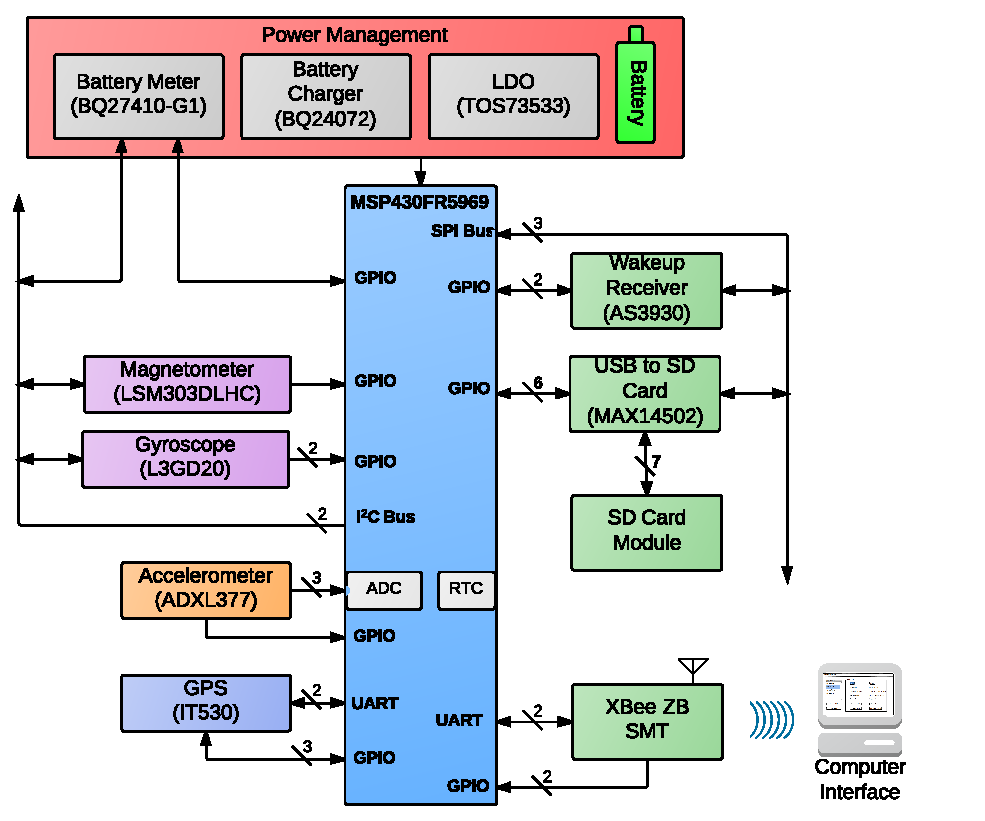
\includegraphics[width=0.95\textwidth]{img/blockDiagram}
	\caption{Revised Block Diagram \label{fig:blockDiagram}}
\end{figure}

%TODO
\todo[inline]{Convert into a shorter paragraph}

\begin{enumerate}
\item Microcontroller
	\begin{itemize}
		\item The microcontroller is needed in order to be able to establish the communication between components, control the different components, and process the output of the sensors.
	\end{itemize}

\item Battery
	\begin{itemize}
		\item A battery is needed because the sphere has to be portable and it is the only way to provide the necessary power.
	\end{itemize}

\item Power Conversion and Management Circuit
	\begin{itemize}
		\item Power Conversion and Management is needed in order to give the necessary and adequate power to each component so that they can work properly and efficiently.  It contains voltage converters and a battery meter.
	\end{itemize}
\item GPS Module
\begin{itemize}
\item A GPS Module is needed in order to know the precise location of the spheres when the user has to recover them after they have been thrown at sea for an experiment.
\end{itemize}
\item Gyroscope
\begin{itemize}
\item The gyroscope will be used to determine the sphere's orientation while being carried by a wave.
\end{itemize}
\item LED
\begin{itemize}
\item An LED will be used to help the user find the sphere when conducting experiments at night and to indicate battery and data transfer status.
\end{itemize}
\item Light Sensor
\begin{itemize}
\item A light sensor will be used in order to only turn on the LED at night to conserve energy.  The LEDs will still display battery and transfer status, but will not flash continuously as would be the case with the LED that aids in finding the spheres at night.
\end{itemize}
\item Real Time Clock
\begin{itemize}
\item A Real Time Clock is needed in this system in order to track and record the time at which each sample measurement is taken in order to be able to match it with the measurements taken by different spheres.
\end{itemize}
\item Accelerometer
\begin{itemize}
\item The accelerometer will be used to measure the acceleration of the sphere while being carried by the waves.
\end{itemize}
\item Analog to Digital Converter (ADC)
\begin{itemize}
\item An ADC is needed in order to take the data from the acceleratometer, which has an analog output, and convert it to digital signals so that the microcontroller can read them.
\end{itemize}
\item SD Card
\begin{itemize}
\item The SD Card will be used to save the data measured during an experiment.
\end{itemize}
\item Wireless Module
\begin{itemize}
\item The wireless module will be used to connect the spheres with a central base so that data can be retrieved without having to open the spheres.
\end{itemize}
\item Computer Interface
\begin{itemize}
\item A computer interface is needed in order to be able to wirelessly retrieve the data collected via wireless and save it for future analysis. 
\end{itemize}

\item Magnetometer
\begin{itemize}
\item Provides the extra 3 degrees of freedom that the researchers need in order to employ dead reckoning algorithms \cite{Canals2012}.
\end{itemize}
\end{enumerate}

